\section{A queueing model with 2 consecutive buffer centres}\label{sec:queueing_model}
% TODO: If this is to be one paper maybe the first two paragraphs do not need to
% include so much details or even better omit some of the details in the game
% overview section.
In this section, a more in-depth explanation of the queueing model shown in 
figure \ref{fig:diagram_of_queueing_system} will be given.
This is a queueing model that consists of two waiting zones, one for each type
of individual.

The model consists of two types of individuals; type 1 and type 2.
Type 1 individuals arrive instantly at waiting zone 1 and wait to receive their 
service. 
Type 2 individuals arrive at waiting zone 2 and wait there until they are 
allowed to move to waiting zone 1. 
They are allowed to proceed only when the number of 
individuals in waiting zone 1 \textbf{and} in service is less than a 
pre-determined threshold \(T\).
When the number of individuals is equal to or exceeds this threshold, all 
second type individuals that arrive will stay 
\textit{blocked} in waiting zone 2 until the number of people in 
the next queue and in service falls below \(T\). 
This is shown diagrammatically in Figure \ref{fig:diagram_of_queueing_system}.
The parameters of the described queueing model are:

\begin{itemize}
    \item \(\lambda_i\): The arrival rate of individuals of type 
    \(i\in\{1, 2\}\)
    \item \(\mu\): The service rate for individuals receiving service
    \item \(C\): The number of servers
    \item \(T\): The threshold at which individuals of the second type are 
    blocked
\end{itemize}

Under the assumption that all rates (arrival and service) are Markovian the
queueing system corresponds to a Markov chain~\cite{kemeny1976markov}.
The states of the Markov chain are denoted by \((u,v)\) where:

\begin{itemize}
    \item \(u\) is the number of individuals blocked
    \item \(v\) is the number of individuals either in waiting zone 1 or in the
    service centre
\end{itemize}

We denote the state space of the Markov chain as  \(S=S(T)\) which can be 
written as the disjoint union (\ref{eq:definition_of_S_as_disjoint_union}).

\begin{align}
    S(T) =& S_1(T) \cup S_2(T) \text{ where:} \nonumber \\
    S_1(T) =& \left\{(0, v)\in\mathbb{N}_0^2 \; | \; v < T \right\} 
    \label{eq:definition_of_S_as_disjoint_union} \\
    S_2(T) =& \{(u, v)\in\mathbb{N}_0^2 \; | \; v \geq T \} \nonumber
\end{align}

The generator matrix \(Q\) of the Markov chain consists of the 
rates between the numerous states of the model. 
Every entry \( Q_{ij} = Q_{(u_i, v_i),(u_j, v_j)} \) represents the rate from 
state \( i = (u_i, v_i) \) to state \( j = (u_j , v_j) \) for all 
\( (u_i, v_i), (u_j, v_j) \in S \).
The entries of \(Q\) can be calculated using the state-mapping function 
described in (\ref{eq:markov_transition_rate}): 

\begin{equation} \label{eq:markov_transition_rate}
    Q_{ij} = 
    \begin{cases}
        \Lambda, & \textbf{if } (u_i, v_i) - (u_j, v_j) = (0,-1) \textbf{ and } 
        v_i < \text{t} \\
        \lambda_1, & \textbf{if } (u_i, v_i) - (u_j, v_j) = (0,-1) 
        \textbf{ and } v_i \geq \text{t} \\
        \lambda_2, & \textbf{if } (u_i, v_i) - (u_j, v_j) = (-1,0) \\
        v_i \mu, & \textbf{if } (u_i, v_i) - (u_j, v_j) = (0,1) \textbf{ and } 
        v_i \leq C \textbf{ or} \\ & \hspace{0.37cm}(u_i, v_i) - (u_j, v_j) = 
        (1,0) \textbf{ and } v_i = T \leq C \\
        C \mu, & \textbf{if } (u_i, v_i) - (u_j, v_j) = (0,1) \textbf{ and } 
        v_i > C 
        \textbf{ or} \\ & \hspace{0.37cm}(u_i, v_i) - (u_j, v_j) = (1,0) 
        \textbf{ and } v_i = T > C\\
        -\sum_{j=1}^{|Q|}{Q_{ij}} & \textbf{if } i = j \\
        0, & \textbf{otherwise}
    \end{cases}
\end{equation}

Note that \(\Lambda\) here denotes the overall arrival rate in the model by both 
types of individuals (i.e. \(\Lambda = \lambda_1 + \lambda_2\)). 
A visualisation of how the transition rates relate to the states of the model 
can be seen in the general Markov chain model shown in Figure 
\ref{fig:general_markov_model}.

\begin{figure}[H]
    \centering
    \scalebox{.8}
    {
        \begin{tikzpicture}[-, node distance = 0.9cm, auto, every node/.style={scale=0.7}]

            % Markov chain variables
            \tikzmath{
                let \initdist = 0.5cm;
                let \altdist = 1.2cm;
                let \minsz = 1.6cm;
            }

            % S_1 and S_2 rectangles
            \tikzmath{
                let \leftOne = -0.8;
                let \rightOne = 2.7;
                let \upOne = 0.8;
                let \downOne = -2.7;
                let \leftTwo = 2.8;
                let \rightTwo = 13;
                let \upTwo = -2.95;
                let \downTwo = -16.4;
            }

            % General case variables
            \tikzmath{
                let \GCsmallx = 8.3;
                let \GCsmally = -9.5;
                let \GCbigx = 4.1;
                let \GCbigy = -11.8;
            }

            % Rectangle for S1
            \draw[ultra thin, dashed] (\leftOne, \downOne) -- (\leftOne, \upOne);
            \draw[ultra thin, dashed] (\leftOne, \upOne) -- (\rightOne, \upOne);
            \draw[ultra thin, dashed] (\rightOne, \upOne) -- node 
            {\Huge{\( \quad S_1 \)}}(\rightOne, \downOne);
            \draw[ultra thin, dashed] (\rightOne, \downOne) -- (\leftOne, \downOne);

            % Rectangle for S2
            \draw[ultra thin, dashed] (\leftTwo, \downTwo) -- node 
            {\Huge{\( S_2 \quad \)}}(\leftTwo, \upTwo);
            \draw[ultra thin, dashed] (\leftTwo, \upTwo) -- (\rightTwo, \upTwo);
            \draw[ultra thin, dashed] (\rightTwo, \upTwo) -- (\rightTwo, \downTwo);
            \draw[ultra thin, dashed] (\rightTwo, \downTwo) -- (\leftTwo, \downTwo);

            % Small square of general case
            \draw [thick] (\GCsmallx, \GCsmally) -- node {} 
            (\GCsmallx + 0.4, \GCsmally);
            \draw [thick] (\GCsmallx + 0.4, \GCsmally) -- node {} 
            (\GCsmallx + 0.4, \GCsmally - 0.4);
            \draw [thick] (\GCsmallx + 0.4, \GCsmally - 0.4) -- node {} 
            (\GCsmallx, \GCsmally - 0.4);
            \draw [thick] (\GCsmallx, \GCsmally - 0.4) -- node {} 
            (\GCsmallx, \GCsmally);


            % Dashed lines to from small square to big one 
            \draw [ultra thin] (\GCsmallx, \GCsmally) -- node {} 
            (\GCbigx, \GCbigy);
            \draw [ultra thin] (\GCsmallx + 0.4, \GCsmally) -- node {} 
            (\GCbigx + 4, \GCbigy);
            \draw [ultra thin] (\GCsmallx, \GCsmally - 0.4) -- node {} (7, \GCbigy);
            \draw [ultra thin] (\GCsmallx + 0.4, \GCsmally - 0.4) -- node {} 
            (\GCbigx + 4, \GCbigy - 4);
            
            % Big Square of general case
            \draw [ultra thick] (\GCbigx, \GCbigy) -- node {} (\GCbigx + 4, \GCbigy);
            \draw [ultra thick] (\GCbigx + 4, \GCbigy) -- node {} 
            (\GCbigx + 4, \GCbigy - 4);
            \draw [ultra thick] (\GCbigx + 4, \GCbigy - 4) -- node {General Case} 
            (\GCbigx, \GCbigy - 4);
            \draw [ultra thick] (\GCbigx, \GCbigy - 4) -- node {} (\GCbigx, \GCbigy);

            % First Line
            \node[state, minimum size=1.5cm] (zero) {(0,0)};
            \node[state, node distance = \initdist, minimum size=\minsz, below right=of zero] 
            (one) {(0,1)};
            \node[draw=none, node distance = \initdist, minimum size=\minsz, below right=of one] 
            (two) {\textbf{\( \ddots \)}};
            \node[state, node distance = \initdist, minimum size=\minsz, below right=of two] 
            (three) {(0,T)};
            \node[state, node distance = \altdist, minimum size=\minsz, right=of three] 
            (four) {(0,T+1)};
            \node[draw=none, node distance = \altdist, minimum size=\minsz, right=of four] 
            (five) {\textbf{\dots}};
            \node[state, minimum size=\minsz, right=of five] (six) {(0,C)};
            \node[draw=none, minimum size=\minsz, right=of six] (seven) {\textbf{\dots}};

            % Second Line
            \node[state, minimum size=\minsz, below=of three] (three_one) {(1,T)};
            \node[state, minimum size=\minsz, below=of four] (four_one) {(1,T+1)};
            \node[draw=none, minimum size=\minsz, below=of five] (five_one) {\textbf{\dots}};
            \node[state, minimum size=\minsz, right=of five_one] (six_one) {(1,C)};
            \node[draw=none, minimum size=\minsz, right=of six_one] (seven_one) {\textbf{\dots}};
            
            % Third Line
            \node[state, minimum size=\minsz, below=of three_one] (three_two) {(2,T)};
            \node[state, minimum size=\minsz, below=of four_one] (four_two) {(2,T+1)};
            \node[draw=none, minimum size=\minsz, below=of five_one] (five_two) 
            {\textbf{\dots}};
            \node[state, minimum size=\minsz, right=of five_two] (six_two) {(2,C)};
            \node[draw=none, minimum size=\minsz, right=of six_two] (seven_two) 
            {\textbf{\dots}};

            % Fourth line
            \node[draw=none, node distance = \altdist, minimum size=\minsz, below=of three_two] 
            (three_three) {\textbf{\vdots}};
            \node[draw=none, node distance = \altdist, minimum size=\minsz, below=of four_two] 
            (four_three) {\textbf{\vdots}};
            \node[draw=none, node distance = 2cm, minimum size=\minsz, below=of five_two] 
            (five_three) {};
            \node[draw=none, node distance = \altdist, minimum size=\minsz, below=of six_two] 
            (six_three) {\textbf{\vdots}};

            % Fifth line
            \node[draw=none, node distance = 0.3cm, minimum size=\minsz, below=of four_three] 
            (general_case_up) {};
            \node[state, node distance = \altdist, minimum size=\minsz, below=of general_case_up] 
            (general_case_mid) {\( (u_i, v_i) \)};

            \node[draw=none, node distance = \altdist, minimum size=\minsz, below=of general_case_mid] 
            (general_case_down) {};
            \node[draw=none, node distance = \altdist, minimum size=\minsz, left=of general_case_mid] 
            (general_case_left) {};
            \node[draw=none, node distance = \altdist, minimum size=\minsz, right=of general_case_mid] 
            (general_case_right) {};

            \draw[every loop]
                % First Horizontal Edges
                (zero) edge[bend left] node {\( \Lambda \)} (one)
                (one) edge[bend left] node {\( \mu \)} (zero)
                (one) edge[bend left] node {\( \Lambda \)} (two)
                (two) edge[bend left] node {\( 2 \mu \)} (one)
                (two) edge[bend left] node {\( \Lambda \)} (three)
                (three) edge[bend left] node {\( T \mu \)} (two)
                (three) edge[bend left] node {\( \lambda_1 \)} (four)
                (four) edge[bend left] node {\( (T+1) \mu \)} (three)
                (four) edge[bend left] node {\( \lambda_1 \)} (five)
                (five) edge[bend left] node {\( (T+2) \mu \)} (four)
                (five) edge[bend left] node {\( \lambda_1 \)} (six)
                (six) edge[bend left] node {\( C\mu \)} (five)
                (six) edge[bend left] node {\( \lambda_1 \)} (seven)
                (seven) edge[bend left] node {\( C\mu \)} (six)

                % Second Horizontal Edges
                (three_one) edge[bend left] node {\( \lambda_1 \)} (four_one)
                (four_one) edge[bend left] node {\( (T+1) \mu \)} (three_one)
                (four_one) edge[bend left] node {\( \lambda_1 \)} (five_one)
                (five_one) edge[bend left] node {\( (T+2) \mu \)} (four_one)
                (five_one) edge[bend left] node {\( \lambda_1 \)} (six_one)
                (six_one) edge[bend left] node {\( C\mu \)} (five_one)
                (six_one) edge[bend left] node {\( \lambda_1 \)} (seven_one)
                (seven_one) edge[bend left] node {\( C\mu \)} (six_one)

                % Third Horizontal Edges
                (three_two) edge[bend left] node {\( \lambda_1 \)} (four_two)
                (four_two) edge[bend left] node [below] {\( (T+1) \mu \)} (three_two)
                (four_two) edge[bend left] node {\( \lambda_1 \)} (five_two)
                (five_two) edge[bend left] node {\( (T+2) \mu \)} (four_two)
                (five_two) edge[bend left] node {\( \lambda_1 \)} (six_two)
                (six_two) edge[bend left] node {\( C\mu \)} (five_two)
                (six_two) edge[bend left] node {\( \lambda_1 \)} (seven_two)
                (seven_two) edge[bend left] node {\( C\mu \)} (six_two)

                % First Vertical Edges
                (three) edge[bend left] node {\( \lambda_2 \)} (three_one)
                (three_one) edge[bend left] node {\( T \mu \)} (three)
                (three_one) edge[bend left] node {\( \lambda_2 \)} (three_two)
                (three_two) edge[bend left] node {\( T\mu \)} (three_one)
                (three_two) edge[bend left] node {\( \lambda_2 \)} (three_three)
                (three_three) edge[bend left] node {\( T\mu \)} (three_two)

                % Second Vertical Edges
                (four) edge node {\( \lambda_2 \)} (four_one)
                (four_one) edge node {\( \lambda_2 \)} (four_two)
                (four_two) edge node {\( \lambda_2 \)} (four_three)

                % Fourth Vertical Edges
                (six) edge node {\( \lambda_2 \)} (six_one)
                (six_one) edge node {\( \lambda_2 \)} (six_two)
                (six_two) edge node {\( \lambda_2 \)} (six_three)

                % General Case
                (general_case_left) edge[bend left] node {\( \lambda_1 \)} (general_case_mid)
                (general_case_mid) edge[bend left] node {\( v_i \mu \)} (general_case_left)
                (general_case_right) edge[bend left] node {\( (v_i +1) \mu \)} (general_case_mid)
                (general_case_mid) edge[bend left] node {\( \lambda_1 \)} (general_case_right)
                % (five_three) edge node {\( \lambda_2 \)} (general_case_mid)
                (general_case_up) edge node {\( \lambda_2 \)} (general_case_mid)
                (general_case_mid) edge node {\( \lambda_2 \)} (general_case_down)
                ;
        \end{tikzpicture}
    }
    \caption{General case of the Markov chain model} 
    \label{fig:general_markov_model}
\end{figure}



In order to consider this model numerically an adjustment needs to be made. 
The problem defined above assumes no upper boundary to the number of individuals 
that can wait for service or for the ones that are blocked in the buffer centre. 
Therefore, a different state space \( \tilde S \) is constructed where 
\( \tilde S \subseteq S \) and there is a maximum allowed number of individuals 
\(N\) that can be in the system and a maximum allowed number of individuals 
\(M\) that can be blocked in the buffer centre:

\begin{equation}
    \tilde S = \left\{ (u, v) \in S\;| u \leq M, v\leq N \right\}
\end{equation}


The generator matrix \( Q \) defined in (\ref{eq:markov_transition_rate}) can 
be used to get the probability vector \( \pi \).
The vector \( \pi \) is commonly used to study stochastic systems and it's main
purpose is to keep track of the probability of being at any given state of 
the system. 
\(\pi_i\) is the steady state probability of being in state \((u_i, v_i) \in 
\tilde S\) which is the \(i^{\text{th}}\) state of \(\tilde S\) for some ordering of 
\(\tilde S\).
The term \textit{steady state} refers to the instance of the vector \( \pi \) 
where the probabilities of being at any state become stable over time. 
Thus, by considering the steady state vector \( \pi \) the relationship between 
it and \( Q \) is given by:

\[
    \frac{d\pi}{dt} = \pi Q = 0
\]

Using vector \(\pi\) there are numerous performance measures of the model that 
can be calculated. 
The following equations utilise \(\pi\) to get performance measures on the 
average number of people at certain sets of state:

\begin{itemize}
    \item Average number of people in the system: 
        \[L = \sum_{i=1}^{|\pi|} \pi_i (u_i + v_i)\]
    \item Average number of people in the service centre: 
        \[L_H = \sum_{i=1}^{|\pi|} \pi_i v_i\]
    \item Average number of people in waiting zone 2:
        \[L_A = \sum_{i=1}^{|\pi|} \pi_i u_i\] 
\end{itemize}

Consequently, there are some additional performance measures of interest that
are not as straightforward to calculate.
Such performance measures are the mean waiting time in the system (for both 
type 1 and type 2 individuals), the mean time blocked in waiting zone 2 (only 
valid for type 2 individuals) and the proportion of individuals that wait in 
waiting zone 1 within a predefined time target (for both types).

\subsection{Waiting time} \label{sec:waiting_time}

Waiting time is the amount of time that patients from either type wait in 
the hospital's waiting space before they can receive their service. 
For a given set of parameters there are three different performance measures 
around the mean waiting time that can be calculated. The mean waiting time of
type 1 individuals:

\begin{equation} \label{eq:closed_form_waiting_type_1}
    W^{(1)} = \frac{\sum_{\substack{(u,v) \, \in S_A^{(1)} \\ v \geq C}} 
    \frac{1}{C \mu} \times (v-C+1) \times \pi(u,v)}{\sum_{(u,v) \, 
    \in S_A^{(1)}} \pi(u,v)}
\end{equation}

The mean waiting time of type 2 individuals:

\begin{equation}\label{eq:closed_form_waiting_type_2}
    W^{(2)} = \frac{\sum_{\substack{(u,v) \, \in S_A^{(2)} \\ min(v,T) \geq C}} 
    \frac{1}{C \mu} \times (\min(v+1,T)-C) \times \pi(u,v)}{\sum_{(u,v) \, 
    \in S_A^{(2)}} \pi(u,v)}
\end{equation} 

The overall mean waiting time:

\begin{equation}\label{eq:overall_waiting_time}
    W = \frac{\lambda_1 P_{L'_1}}{\lambda_2 P_{L'_2} + \lambda_1 P_{L'_1}} W^{(1)} 
    + \frac{\lambda_2 P_{L'_2}}{\lambda_2 P_{L'_2} + \lambda_1 P_{L'_1}} W^{(2)}
\end{equation}
 
Here \(S_A^{(1)}\) and \(S_A^{(2)}\) are the set of accepting states for type
1 and type 2 individuals. These are the set of states that the model is able
to accept a specific type of individuals.

\begin{equation}\label{eq:accepting_states_type_1}
    S_A^{(1)} = \{(u, v) \in S \; | \; v < N \}
\end{equation}

\begin{equation}\label{eq:accepting_states_type_2}
    S_A^{(2)}=
    \begin{cases}
        \{(u, v) \in S \; | \; u < M \}, & \textbf{if } T \leq N\\
        \{(u, v) \in S \; | \; v < N \}, & \textbf{otherwise}
    \end{cases}
\end{equation}

Equation \ref{eq:overall_waiting_time} makes use of the proportion of type 1 
and type 2 individuals that are not lost to the system. These probabilities are 
given by \(P_{L'_1}\) and \(P_{L'_2}\) where:

\begin{equation}\label{eq:proportion_of_accepting_individuals}
    P_{L'_1} = \sum_{(u,v) \, \in S_A^{(1)}} \pi(u,v) \hspace{2cm}
    P_{L'_2} = \sum_{(u,v) \, \in S_A^{(2)}} \pi(u,v)
\end{equation}
 
Appendix \ref{sec:appendix_mean_waiting} gives more details on the recursive
formula that equations (\ref{eq:closed_form_waiting_type_1}),
(\ref{eq:closed_form_waiting_type_2}) and (\ref{eq:overall_waiting_time})
originate from. 

Figure \ref{fig:markov_vs_des_waiting_time_comparison_overall} shows a 
comparison between the calculated mean waiting time using Markov chains and the
simulated waiting time using discrete event simulation over a range of values of 
\(\lambda_2\) (details of the discrete event simulation model are given in 
appendix~\ref{sec:appendix_des}).
The simulation was ran 100 times and the recorded mean waiting time at each 
iteration is used to populate the violin plots.
The waiting times generated by the simulation match the ones generated by the 
Markov chains model.
Note that this comparison includes both type 1 and type 2 individuals.
A separate comparison of only type 1 and only type 2 individuals can be found 
in appendix~\ref{sec:appendix_additional_figures}.

\begin{figure}[H]
    \centering
    \includegraphics[width=.8\textwidth]{imgs/waiting_time_comparison/waiting_overall.pdf}
    \caption{
        Comparison of mean waiting time for both types of individuals between 
        values obtained from the Markov chain formulas and values obtained from 
        simulation.
    }
    \label{fig:markov_vs_des_waiting_time_comparison_overall}
\end{figure}


\subsection{Blocking time}\label{sec:blocking_time}

% TODO: Possibly replace the contents of this section with the ones for the 
% closed form formula of the blocking time
% Currently the direct approach one is shown

Blocking time is the amount of time that type 2 patients wait in the parking 
space before they are allowed to proceed to the hospital.
Unlike the waiting time, the blocking time is only calculated for type 2 
individuals.  
That is because type 1 individuals cannot be blocked. 
Thus, one only needs to consider the pathway of type 2 individuals to get the 
mean blocking time of the system. 
The mean blocking time can by calculated using:

\begin{equation}\label{eq:algebraic_blocking_time}
    B = \frac{\sum_{(u,v) \in S_A^{(2)}} \pi_{(u,v)} \; 
    b(\mathcal{A}_2(u,v))}{\sum_{(u,v) \in S_A^{(2)}} \pi_{(u,v)}}
\end{equation}

Here \(S_A^{(2)}\) is the set of accepting states of type 2 individuals (defined
in equation (\ref{eq:accepting_states_type_2})) and \(\mathcal{A}_i(u,v)\) for
\(i \in \{1, 2\} \) is the state that the system would go to when the system is
at state \( (u,v) \) and an individual of type \(i\) arrives. 

\begin{equation}\label{eq:arriving_state_class_1}
    \mathcal{A}_1(u,v) = (u, v + 1)
\end{equation}
\begin{equation}\label{eq:arriving_state_class_2}
    \mathcal{A}_2(u,v) = 
    \begin{cases}
        (u, v + 1), & \text{if } v < T \\
        (u + 1, v), & \text{if } v \geq T \\
    \end{cases}
\end{equation}

The term \(b(u,v)\) is the mean time that an individual will be blocked for, 
when the individual arrives in the system at state \((u,v)\). 
For all the states of the system \(b(u,v)\) is given by:

\begin{equation}\label{eq:general_blocking_time_at_each_state}
    b(u,v) = 
    \begin{cases} 
        0, & \textbf{if } (u,v) \notin S_b \\
        c(u,v) + b(u - 1, v), & \textbf{if } v = N = T\\
        c(u,v) + b(u, v-1), & \textbf{if } v = N \neq T \\
        c(u,v) + p_s(u,v) b(u-1, v) + p_a(u,v) b(u, v+1), & \textbf{if } u > 0 
        \textbf{ and } \vspace{-0.2cm} \\ 
        & \quad v = T \\
        c(u,v) + p_s(u,v) b(u, v-1) + p_a(u,v) b(u, v+1), & \textbf{otherwise} \\
    \end{cases}
\end{equation}

Note that \(S_b\) is defined as the set of states where individuals can be
blocked and is given by:

\begin{equation} \label{eq:set_of_blocking_states}
    S_b = \{(u,v) \in S \; | \; u > 0\}
\end{equation}

Additionally, \(c(u,v)\) is the mean sojourn time for each state and \(p_s\) 
and \(p_a\) are the probabilities that the next event to occur will be a 
service completion or an arrival of a type 1 individual:

\begin{equation}\label{eq:sojourn_blocking_time}
    c(u,v) = 
    \begin{cases}
        \frac{1}{\min(v,C) \mu}, & \text{if } v = N\\
        \frac{1}{\lambda_1 + \min(v,C) \mu}, & \text{otherwise}
    \end{cases}
\end{equation}

\begin{equation}\label{eq:probs_of_service_and_arrival}
    p_s(u,v) = \frac{\min(v,C)\mu}{\lambda_1 + \min(v,C)\mu}, \qquad
    p_a(u,v) = \frac{\lambda_1}{\lambda_1 + \min(v,C)\mu}
\end{equation}

The system of equations produced by 
(\ref{eq:general_blocking_time_at_each_state}) can be solved by considering the 
linear system \(Zx=y\). 
Assuming \(i\) and \(j\) represent states \((u_i, v_i), (u_j, v_j) \in S_b\) 
then \(Z_{ij}\) is given by:

\begin{equation}\label{eq:general_mapping_function_of_blocking_matrix}
    Z_{ij} = 
    \begin{cases}
        p_a, & \textbf{if } j = i + 1 \textbf{ and } v_i \neq N \\
        p_s, & \textbf{if } j = i - 1 \textbf{ and } v_i \neq N, v_i \neq T \\
             & \textbf{or } j = i - N + T \textbf{ and } u_i \geq 2,\,v_i = T \\
        1, & \textbf{if } j = i - 1 \textbf{ and } v_i = N \\
        -1, & \textbf{if } i = j \\
        0, & \textbf{otherwise} \\
    \end{cases}
\end{equation}

Equation~(\ref{eq:general_algebaric_approach_blocking_time}) shows this.
\begin{equation}\label{eq:general_algebaric_approach_blocking_time}
    \scalebox{0.73}{\(
        Z = 
        \begin{pmatrix}
            -1 & p_a & 0 & \dots & 0 & 0 & 0 & 0 & 0 & \dots & 0 & 0 \\ %(1,T)
            p_s & -1 & p_a & \dots & 0 & 0 & 0 & 0 & 0 & \dots & 0 & 0 \\ %(1,T+1)
            0 & p_s & -1 & \dots & 0 & 0 & 0 & 0 & 0 & \dots & 0 & 0 \\ %(1,T+2)
            \vdots & \vdots & \vdots & \ddots & \vdots & \vdots & \vdots & 
            \vdots & \vdots & \ddots & \vdots & \vdots \\ 
            0 & 0 & 0 & \dots & 1 & -1 & 0 & 0 & 0 & \dots & 0 & 0 \\ %(1,N)
            p_s & 0 & 0 & \dots & 0 & 0 & -1 & p_a & 0 & \dots & 0 & 0 \\ %(2,T)
            0 & 0 & 0 & \dots & 0 & 0 & p_s & -1 & p_a & \dots & 0 & 0 \\ %(2,T+1)
            \vdots & \vdots & \vdots & \ddots & \vdots & \vdots & \vdots & 
            \vdots & \vdots & \ddots & \vdots & \vdots \\ 
            0 & 0 & 0 & \dots & 0 & 0 & 0 & 0 & 0 & \dots & 1 & -1 \\ %(M,N)
        \end{pmatrix},
        x = 
        \begin{pmatrix}
            b(1,T) \\
            b(1,T+1) \\
            b(1,T+2) \\
            \vdots \\
            b(1,N) \\
            b(2,T) \\
            b(2,T+1) \\
            \vdots \\
            b(M,N) \\
        \end{pmatrix}, 
        y= 
        \begin{pmatrix}
            -c(1,T) \\
            -c(1,T+1) \\
            -c(1,T+2) \\
            \vdots \\
            -c(1,N) \\
            -c(2,T) \\
            -c(2,T+1) \\
            \vdots \\
            -c(M,N) \\
        \end{pmatrix}
    \)}
\end{equation}


Additional details on the blocking time formula 
(\ref{eq:algebraic_blocking_time}) can be found in appendix 
\ref{sec:appendix_mean_blocking}. 

Figure \ref{fig:markov_vs_des_blocking_time_comparison} illustrates a comparison 
between the formulas that arise from the Markov chain model and the equivalent 
values of the blocking time extracted from discrete event simulation
(appendix~\ref{sec:appendix_des}).
The blocking time is calculated using both methods for a range of values of
\(\lambda_2\).
The figure is used to demonstrate the accuracy of the blocking time formula of
the constructed queueing model as well as the effect of truncating the model.
The simulation was ran 100 times and the recorded mean blocking time at each 
iteration is used to populate the violin plots.
Similar to figure \ref{fig:markov_vs_des_waiting_time_comparison_overall}, these
plots shows a comparison between the calculated mean blocking time using Markov 
chain, using a truncated simulation and using a simulation with infinite
capacity (without the artificial parameters \(N\) and \(M\)).
The blocking times generated by the truncated simulation match the ones
generated by the Markov chains model.
Note that this comparison includes just type 2 individuals since type 1 
individuals cannot be blocked.

\begin{figure}[H]
    \centering
    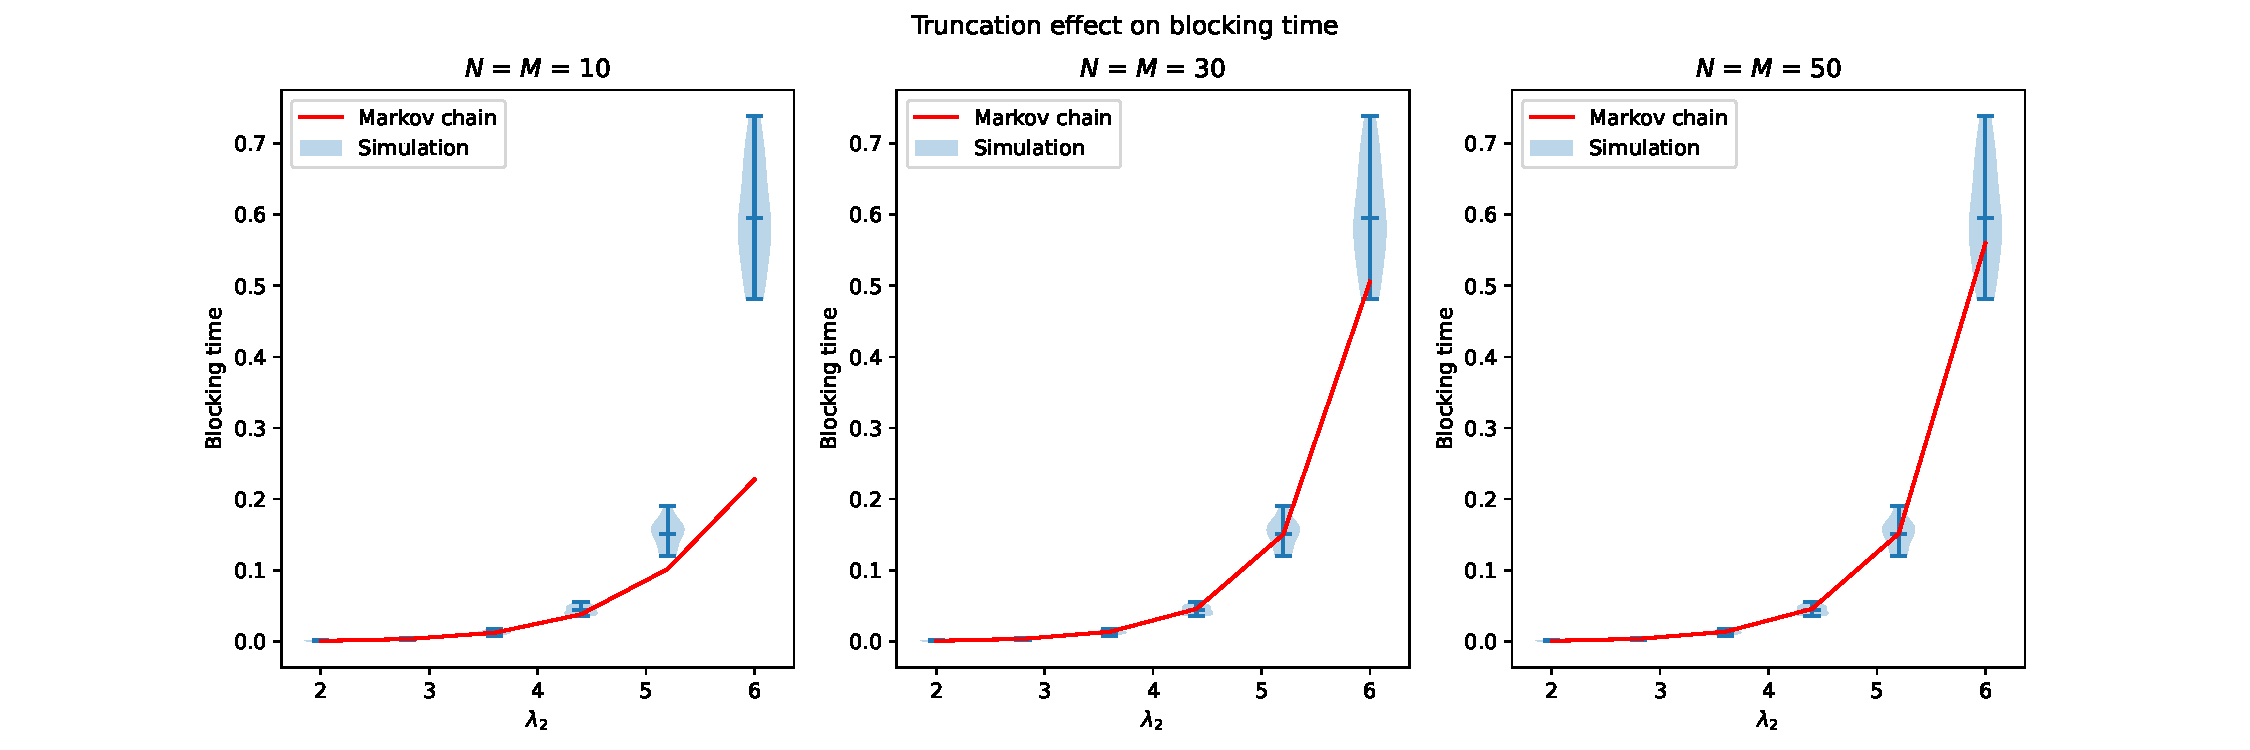
\includegraphics[width=\textwidth]{imgs/truncation_effect/blocking/main.pdf}
    \caption{
        Comparison of mean blocking time between values obtained from the Markov 
        chain formula, values obtained from the truncated simulation and values
        obtained from the untruncated simulation.
    }
    \label{fig:markov_vs_des_blocking_time_comparison}
\end{figure}


\subsection{Proportion of individuals within target}\label{sec:proportion_within_target}

Another performance measure that is taken into consideration is the proportion 
of individuals whose time in the hospital (waiting and service time) is within
a specified time target \(t\).
Similar to section \ref{sec:waiting_time}, three formulas are needed for this 
performance measure.

The proportion of type 1 individuals within a time target:

\begin{equation}\label{eq:proportion_within_target_type_1}
    P(X^{(1)} < t) = \frac{\sum_{(u,v) \in S_A^{(1)}} 
    P(X_{\mathcal{A}_1(u,v)}^{(1)} < t) 
    \pi_{u,v} }{\sum_{(u,v) \in S_A^{(1)}} \pi_{u,v}}
\end{equation}

The proportion of type 2 individuals within a time target:

\begin{equation}\label{eq:proportion_within_target_type_2}
    P(X^{(2)} < t) = \frac{\sum_{(u,v) \in S_A^{(2)}} 
    P(X_{\mathcal{A}_2(u,v)}^{(2)} < t) 
    \pi_{u,v} }{\sum_{(u,v) \in S_A^{(2)}} \pi_{u,v}}
\end{equation}

The terms \(\mathcal{A}_1(u,v)\) and \(\mathcal{A}_2(u,v)\) are defined by
equations \ref{eq:arriving_state_class_1} and \ref{eq:arriving_state_class_2}
in section \ref{sec:blocking_time}.
The overall proportion individuals within a time target (where \(P_{L'_1}\) and 
\(P_{L'_1}\) are defined in (\ref{eq:proportion_of_accepting_individuals})):

\begin{equation}\label{eq:overall_proportion_within_target}
    P(X < t) = \frac{\lambda_1 P_{L'_1}}{\lambda_2 P_{L'_2}+\lambda_1 P_{L'_1}} 
    P(X^{(1)} < t) + \frac{\lambda_2 P_{L'_2}}{\lambda_2 P_{L'_2} + 
    \lambda_1 P_{L'_1}} P(X^{(2)} < t) 
\end{equation}

Here \(P(X_{(u,v)}^{(1)})\) and \(P(X_{(u,v)}^{(2)})\) are defined as the
proportion of individuals within the time target \(t\) when starting from state 
\((u,v)\).
These expression can be calculated by:

\begin{equation}\label{eq:proportion_within_target_type_1_from_state}
    P(X_{(u,v)}^{(1)} < t) = 
    \begin{cases}
        1 - \sum_{i=0}^{v-1} \frac{1}{i!} e^{-\mu t} (\mu t)^i, 
            & \textbf{if } C = 1 \\
            & \textbf{and } v>1 \\
        1 - (\mu C)^{v-C} \mu  
            \sum_{k=1}^{\mid \vec{r} \mid} \sum_{l=1}^{r_k}
            \frac{\Psi_{k,l}(-\lambda_k)t^{r_k - l} 
            e^{-\lambda_k t}}{(r_k - l)! (l - 1)!},
            & \textbf{if } C > 1 \\
            & \textbf{and } v > C \\
        1 - e^{-\mu t},  & \textbf{if } v \leq C
    \end{cases}
\end{equation}

\noindent
where \(\vec{r}=(v - C, 1)\), \(\vec{\lambda}=(C \mu, \mu)\) and 
\(\lambda_0 = 0, r_0\) = 1. 

\begin{equation}\label{eq:proportion_within_target_type_2_from_state}
    P(X_{(u,v)}^{(2)} < t) = 
    \begin{cases}
        1 - \sum_{i=0}^{\min(v,T)-1} \frac{1}{i!} e^{-\mu t} (\mu t)^i,  
            & \textbf{if } C = 1 \\ 
            & \textbf{and } v, T > 1 \\
        1 - (\mu C) ^ {\min(v,T) - C} \mu  
        \sum_{k=1}^{\mid \vec{r} \mid} & \textbf{if } C > 1 \\
        \qquad \times \sum_{l=1}^{r_k}
        \frac{\Psi_{k,l}(-\lambda_k)t^{r_k - l} 
        e^{-\lambda_k t}}{(r_k - l)! (l - 1)!}, 
            & \textbf{and } v, T  > C\\
        1 - e^{-\mu t}, & \textbf{if } v \leq C \\ 
            & \textbf{or } T \leq C \\
    \end{cases}
\end{equation}

\noindent
where \(\vec{r}=(\min(v, T) - C, 1)\), \(\vec{\lambda}=(C \mu, \mu)\) and
\(\lambda_0 = 0, r_0 = 1\).


The function \(\Psi_{k,l}\) used in equations 
(\ref{eq:proportion_within_target_type_1_from_state}) and 
(\ref{eq:proportion_within_target_type_2_from_state}) is defined as:

\begin{equation}
    \Psi_{k,l}(t) = 
    \begin{cases} 
        \frac{(-1)^{l} (l-1)!}{\lambda_2} \left[\frac{1}{t^l} - \frac{1}
        {(t + \lambda_2)^l}\right] , & k=1 \\
        - \frac{1}{t (t + \lambda_1)^{r_1}}, & k=2
    \end{cases} \nonumber \\
\end{equation}

Please refer to appendix \ref{sec:appendix_mean_proportion} for a more in-depth 
explanation of the origins of equations 
(\ref{eq:proportion_within_target_type_1}) - 
(\ref{eq:proportion_within_target_type_2_from_state}).

Figure \ref{fig:markov_vs_des_proportion_comparison_overall} shows a comparison
of the mean proportion of individuals within target when using Markov chains 
and discrete event simulation (appendix~\ref{sec:appendix_des}).
The figure is used to demonstrate the accuracy of the formula for the 
proportion of individuals within time of the constructed queueing model
as well as the effect that truncating the model has on the formula.
The simulation was ran 100 times and the recorded proportions at each iteration 
is used to populate the violin plots.
Similar to figures \ref{fig:markov_vs_des_waiting_time_comparison_overall} and
\ref{fig:markov_vs_des_blocking_time_comparison}, these plots shows a comparison
between the calculated mean proportion of individuals within time using Markov 
chain, using a truncated simulation and using a simulation 
without the artificial parameters \(N\) and \(M\).
The proportions generated by the truncated simulation match the ones generated
by the Markov chains model.
Note that this comparison includes both type 1 and type 2 individuals.
A separate comparison of only type 1 and only type 2 individuals can be found 
in appendix~\ref{sec:appendix_additional_figures}.

\begin{figure}[H]
    \centering
    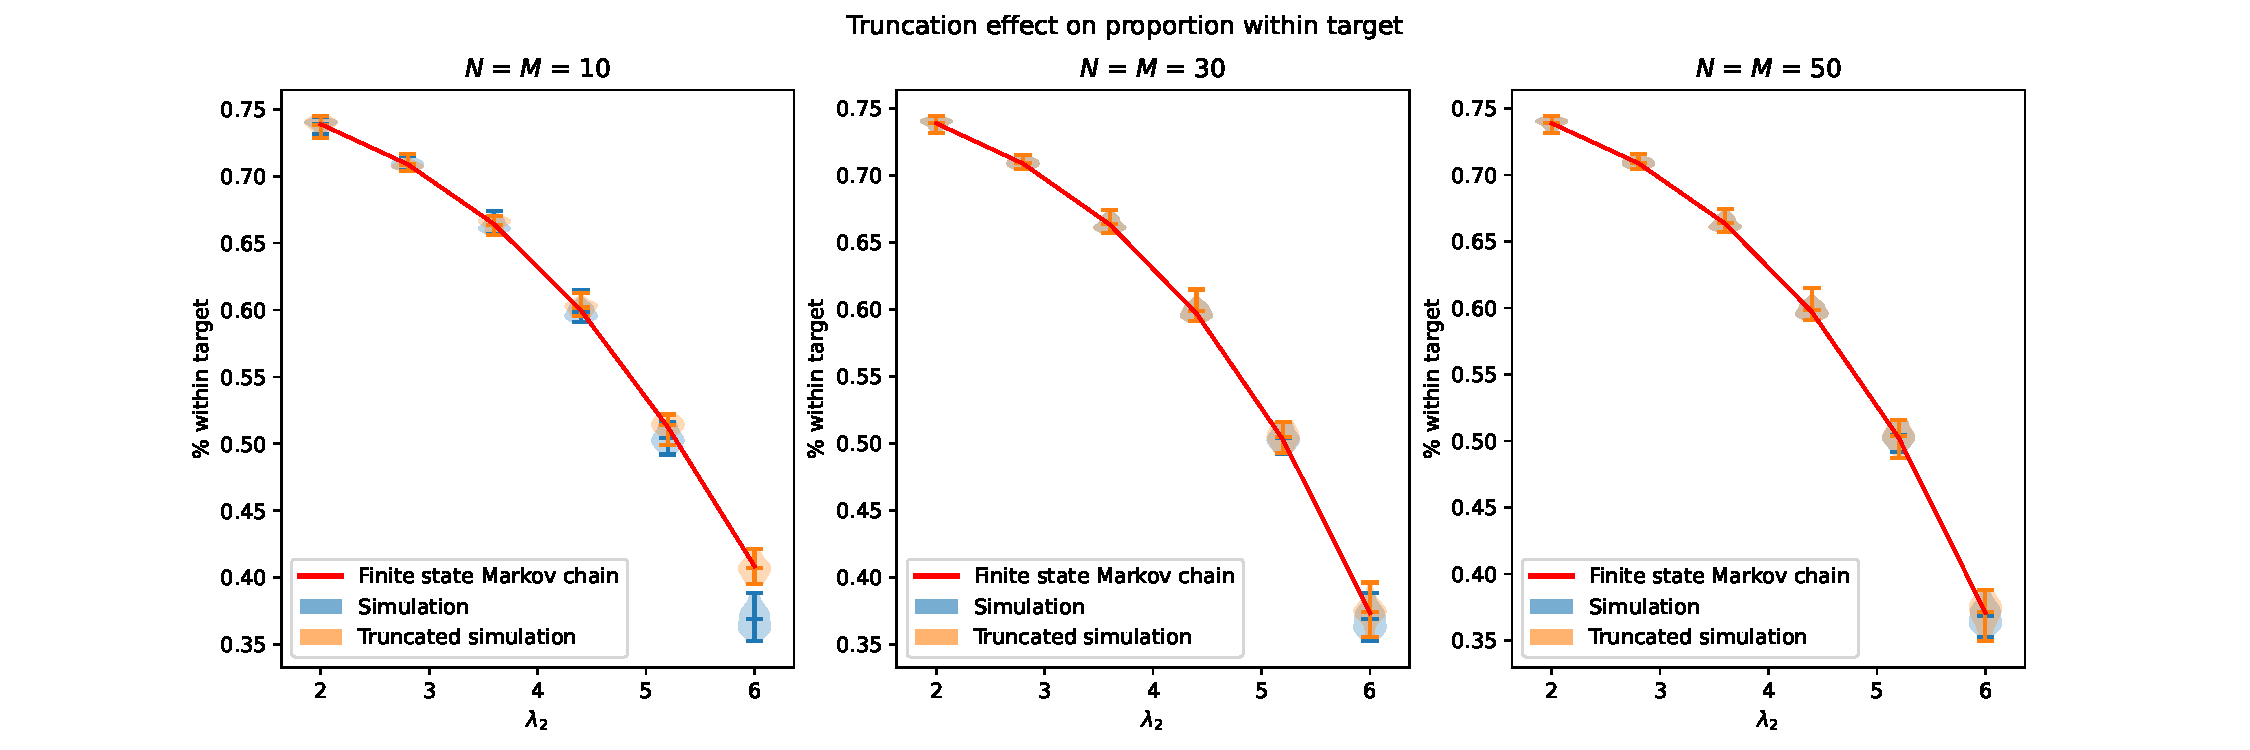
\includegraphics[width=\textwidth]{imgs/truncation_effect/proportion/main.pdf}
    \caption{
        Comparison of mean proportion of individuals within target time between 
        values obtained from the Markov chain formula, values obtained from the
        truncated simulation and values obtained from the untruncated
        simulation. 
    }
    \label{fig:markov_vs_des_proportion_comparison_overall}
\end{figure}
